\documentclass[11pt]{beamer}
%\usetheme{plain}
\usepackage[utf8]{inputenc}
\usepackage{amsmath}
\usepackage{amsfonts}
\usepackage{amssymb}
\usepackage{tikz}
\usetikzlibrary{arrows}
 
\begin{document}

\begin{frame}{The SimulAI framework: an overview}

\begin{itemize} 
	\item At this stage of development, the library is intended to reduce the work involved in coding machine-learning applications and not automate the entire process.
	\item In other words, the user is considered able of handling the software in a lower level in order to construct applications. 
	\item  Nonetheless, the automation feature can be encompassed in due course.
\end{itemize}	
	 
\end{frame}

\begin{frame}{The SimulAI framework: training process}

	\scalebox{0.64}{
	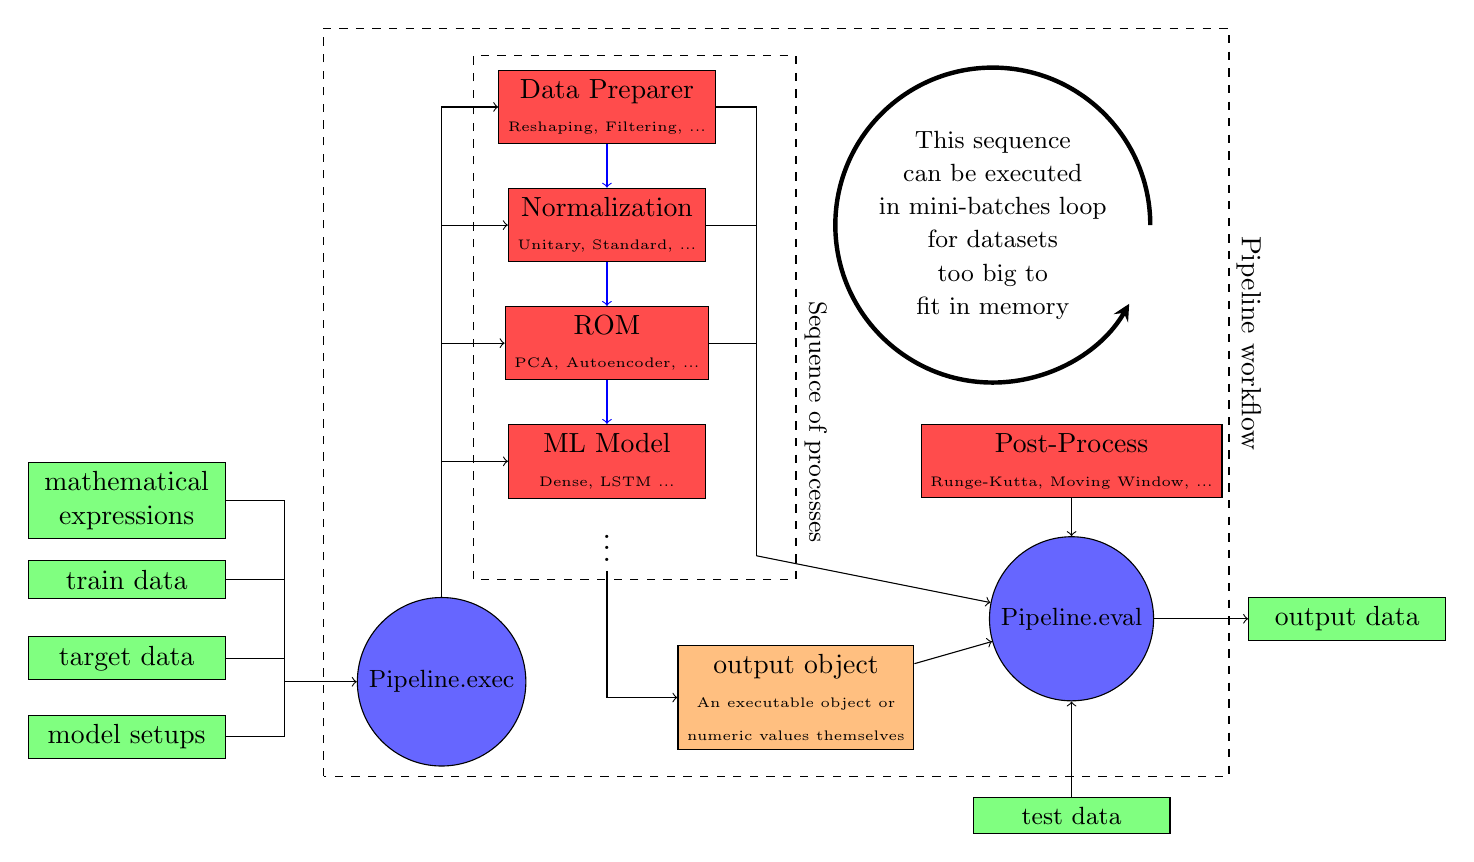
\begin{tikzpicture}
		
	\tikzstyle{class_node}=[circle, fill=blue!60, draw=black]
	\tikzstyle{dependency_node}=[rectangle, fill=green!50, minimum width=25mm, draw=black]
	\tikzstyle{auxiliary_class_node}=[rectangle, fill=red!70, minimum width=25mm, draw=black]
	\tikzstyle{special_arrow}=[->, draw=blue] 
	\tikzstyle{logical_symbol}=[circle, fill=blue!30, draw=black]
	\tikzstyle{object_node}=[rectangle, fill=orange!50, minimum width=25mm, draw=black]
	%Main nodes 
	\node[dependency_node] at (-1., 2) (input) {train data};
	\node[dependency_node] at (-1., 1) (target) {target data};
	\node[dependency_node] at (-1., 0) (model_setups) {model setups};
	\node[dependency_node, align=center] at (-1., 3) (math_expr) {mathematical\\ expressions};
	
	\node[auxiliary_class_node, align=center] at (5.1, 8.) (data_preparer) {Data Preparer \\\tiny{Reshaping, Filtering, ...}};
	\node[auxiliary_class_node, align=center] at (5.1, 6.5) (normalization) {Normalization \\ \tiny{Unitary, Standard, ...}};
 	\node[auxiliary_class_node, align=center] at (5.1, 5.)  (rom) {ROM\\ \tiny{PCA, Autoencoder,  ...}};
	\node[auxiliary_class_node, align=center] at (5.1, 3.5) (model) {ML Model\\ \tiny{Dense, LSTM ...}};
	\node[] at (5.1, 2.5) (etc) {\large \vdots};
	
	\coordinate (reference_input) at (1., .7);
	\coordinate (reference_output) at (12.55, 1.5);
	
	\node[class_node] at (3, .7) (pipeline) {\small Pipeline.exec};
	\node[object_node, align=center] at (7.5, .5) (output) {output object\\ \tiny{An executable object or}\\ \tiny{numeric values themselves}};
	\node[class_node] at (11, 1.5) (pipeline_eval) {\small Pipeline.eval};
	\node[dependency_node] at (11, -1) (test_data) {\small test data};
	\node[dependency_node] at (14.5, 1.5) (another_output_data) {output data};
	\node[auxiliary_class_node, align=center] at (11, 3.5) (post_process) {Post-Process\\ \tiny{Runge-Kutta, Moving Window, ...}};
	\coordinate (reference) at (7, 2.3);
	
	% Text nodes
	\node[align=right, rotate=-90] at (7.75, 4) {\small Sequence of processes};
	
	% Connections
	
	\draw[] (math_expr) -| (reference_input);
	\draw[] (input) -| (reference_input);
	\draw[] (model_setups) -| (reference_input);
	\draw[] (target) -| (reference_input);
	\draw[->] (reference_input) -- (pipeline); 
	
	\draw[dashed] (3.4, 2) rectangle (7.5,8.65);
	
	\draw[->] (pipeline) |- (data_preparer) ;
	\draw[->] (pipeline) |- (normalization);
	\draw[->] (pipeline) |- (rom);
	\draw[->] (pipeline)  |-(model) ;	
	
	\draw[special_arrow] (data_preparer) -- (normalization);
	\draw[special_arrow](normalization) -- (rom);
	\draw[special_arrow] (rom) -- (model);
	%\draw[special_arrow] (model) -- (etc);
	
	\draw[->] (etc) |- (output);
	%\draw[->] (or) -- (output);
	%\draw[->] (or) -- (output_data);
	
	\draw[->] (output) -- (pipeline_eval);
	\draw[] (pipeline_eval) -- (reference_output);
	\draw[->] (pipeline_eval) -- (another_output_data);
	\draw[->] (post_process) -- (pipeline_eval);
	
	\draw[] (data_preparer) -| (reference);
	\draw[] (normalization) -| (reference);
	\draw[] (rom) -| (reference);
	\draw[->] (reference) -- (pipeline_eval);
	\draw[->] (test_data) -- (pipeline_eval);
	
	\node[align=center] at (10., 6.5) (center) {\small{This sequence}\\ \small{can be executed}\\ \small{in mini-batches loop}\\ \small{for datasets}\\ \small{too big to}\\ \small{fit in memory}};
	\draw[ultra thick, ->,>=stealth] (12, 6.5) arc[radius=2.0cm,start angle=0,delta angle=330];
	
	\draw[dashed] (1.5, -.5) rectangle (13.,9);
	\node[align=center, rotate=-90] at (13.25, 5) {Pipeline workflow};
	\end{tikzpicture}
	}
\end{frame}

\begin{frame}{The SimulAI framework: The construction of the machine learning model}
	
	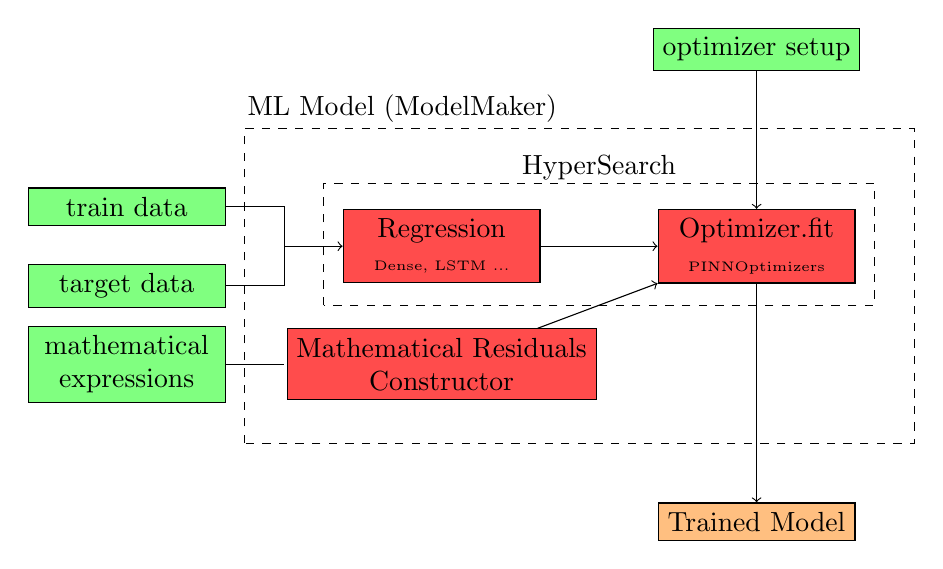
\begin{tikzpicture}
	
	\tikzstyle{class_node}=[circle, fill=blue!60, draw=black]
	\tikzstyle{dependency_node}=[rectangle, fill=green!50, minimum width=25mm, draw=black]
	\tikzstyle{auxiliary_class_node}=[rectangle, fill=red!70, minimum width=25mm, draw=black]
	\tikzstyle{special_arrow}=[->, draw=blue] 
	\tikzstyle{logical_symbol}=[circle, fill=blue!30, draw=black]
	\tikzstyle{object_node}=[rectangle, fill=orange!50, minimum width=25mm, draw=black]
	
	\coordinate (reference_input_1) at (1., 2.5);
	\coordinate (reference_input_2) at (1., 1);
	
	\node[dependency_node] at (-1., 3) (input) {train data};
	\node[dependency_node] at (7., 5) (optimizer_setup) {optimizer setup};
	\node[dependency_node] at (-1., 2) (target) {target data};
	\node[dependency_node, align=center] at (-1., 1) (math_expr) {mathematical\\ expressions};
	
	\node[auxiliary_class_node, align=center] at (3, 2.5) (regression) {Regression\\ \tiny{Dense, LSTM ...}};
	\node[auxiliary_class_node, align=center] at (3, 1) (residuals_construction) {Mathematical Residuals\\ Constructor};

	\node[auxiliary_class_node, align=center] at (7, 2.5) (optimizer) {Optimizer.fit \\ \tiny{PINNOptimizers}};
	
	\node[object_node] at (7, -1) (trained_model) {Trained Model}; 
	
	\node[] at (2.5, 4.25) {ML Model (ModelMaker)};
	\draw[] (input) -| (reference_input_1);
	\draw[] (target) -| (reference_input_1);
	\draw[] (math_expr) -| (reference_input_2);
	\draw[->] (reference_input_1) -- (regression);
	\draw[->] (regression) -- (optimizer);
	\draw[->] (residuals_construction) -- (optimizer);
	\draw[->] (optimizer_setup) -- (optimizer);
	\draw[->] (optimizer) -- (trained_model);
	
	\draw[dashed] (0.5, 0) rectangle (9, 4);
	\draw[dashed] (1.5, 1.75) rectangle (8.5, 3.3);
	\node[] at  (5, 3.5) {HyperSearch};
	\end{tikzpicture}
	
\end{frame}


\end{document}